\chapter{Projekt systemu}
W~tym rozdziale zdecyduję, jaką ścieżką pójdę, aby stworzyć oprogramowanie realizujące cele opisane w~punkcie~\ref{lib-requirements}.
Ta decyzja będzie poprzedzona zebraniem wymagań i~prototypowaniem.
Po niej nastąpi szczegółowe projektowanie i~w~końcu implementacja mojego rozwiązania.

%\section{Wybór metodyki}
%Mógłbym tutaj przedstawić po co w~ogóle są metodyki wytwarzania oprogramowania, przeanalizować najpopularniejsze i~jakąś wybrać, pewnie dostosowując jeszcze do swoich potrzeb.
%Np. na początku podział na zwinne i nie. Mi oczywiście pasują zwinne, bo nie jestem gigantycznym projektem. Poza tym zwinne są lepsze i RUP to tylko nieudana teoria.
%Potem powiedzieć, co to Scrum i że nie potrzebuje, bo nie mam zespołu.
%Potem Extreme Programming przedstawić, i powiedzieć, że ma Spajki, a to jest coś, co mi się przyda.
%Jakieś linki do tego:
%http://servicevirtualization.com/profiles/blogs/when-agile-is-not-enough
%https://www.scrum.org/resources/what-is-scrum/

%\section{Metodyka wytwarzania(TODO)}
%Zdecydowałem, że tworząc mój projekt będę postępował zgodnie Zabierając się za projekt informatyczny dobrze sobie obrać jakąś metodykę (źródło).
%Ja zdecydowałem się na pewną wersję Xtreme programming.
%Jeśli będę robił jakieś większe schematy to będzie to zapożyczenie z~cięższych metodyk, niejako potrzebne dla naukowego aspektu pracy.

\section{Specyfikacja wymagań systemowych (SWS)}
\textbf{TOOOOODOOOOOO}
Z~celów tej pracy zawartych w~punkcie~\ref{lib-requirements} stworzyłem standardową listę konkretnych wymagań dla zespołu inżynierów, czyli mnie samego.
Tworząc niniejszą sekcję wzorowałem się na specyfikacji wymagań systemowych opisanej w~prezentacji ,,Inżynieria Wymagań'' Jarosława Kuchty, z~przedmiotu ,,Dokumentacja i~Jakość Oprogramowania''. (dodać do źródeł) (\url{http://galaxy.eti.pg.gda.pl/katedry/kask/pracownicy/Jaroslaw.Kuchta/DJO/04.InzynieriaWymagan.ppt}).


\subsection{Wstęp i~opis informacyjny}
Jako rozbudowana sekcja wstępu SWS oraz ,,szczegółowy opis problemów do rozwiązania'' służyły poprzednie rozdziały niniejszej pracy.

%http://tex.stackexchange.com/questions/26484/whats-the-best-way-to-embed-visio-diagrams
\subsubsection{Diagram przepływu najwyższego poziomu(TODO)}
Diagram~\ref{fig:project-overview} przedstawia ogólną wizję projektu.
Latają sobie obiekty i wywołania. Wszystko to polimorficzne.
Takie przejście przez system.

Po obu stronach są te same typy, generowane jedne z drugich. Przez to może dobrze działać polimorfizm. Typy wygenerowane oznaczone apostrofem (typ prim).
Serwer może zebrać kilka obiektów, wystawiać ich metody na zewnątrz i przyjmować żądania wywołania na nich metod.
Każdy z tych obiektów musi spełniać jakiś interfejs. Ten interfejs musi być przetłumaczony dla drugiej strony, która zrobi wtedy na jego bazie zdalny obiekt.
Klientów można tworzyć kilka. Klient jest generowany przez mój kod, ale spełnia jakiś zadany interfejs.
Wszystko leci przez jakiś kanał komunikacyjny. Musi on być dwustronny. Nie ma na to jakiś ograniczeń. Musi wspierać wysyłanie wiadomości (paczek danych). Może to być TCP, HTTP, SSL, cokolwiek.

\begin{figure}
	\centering
		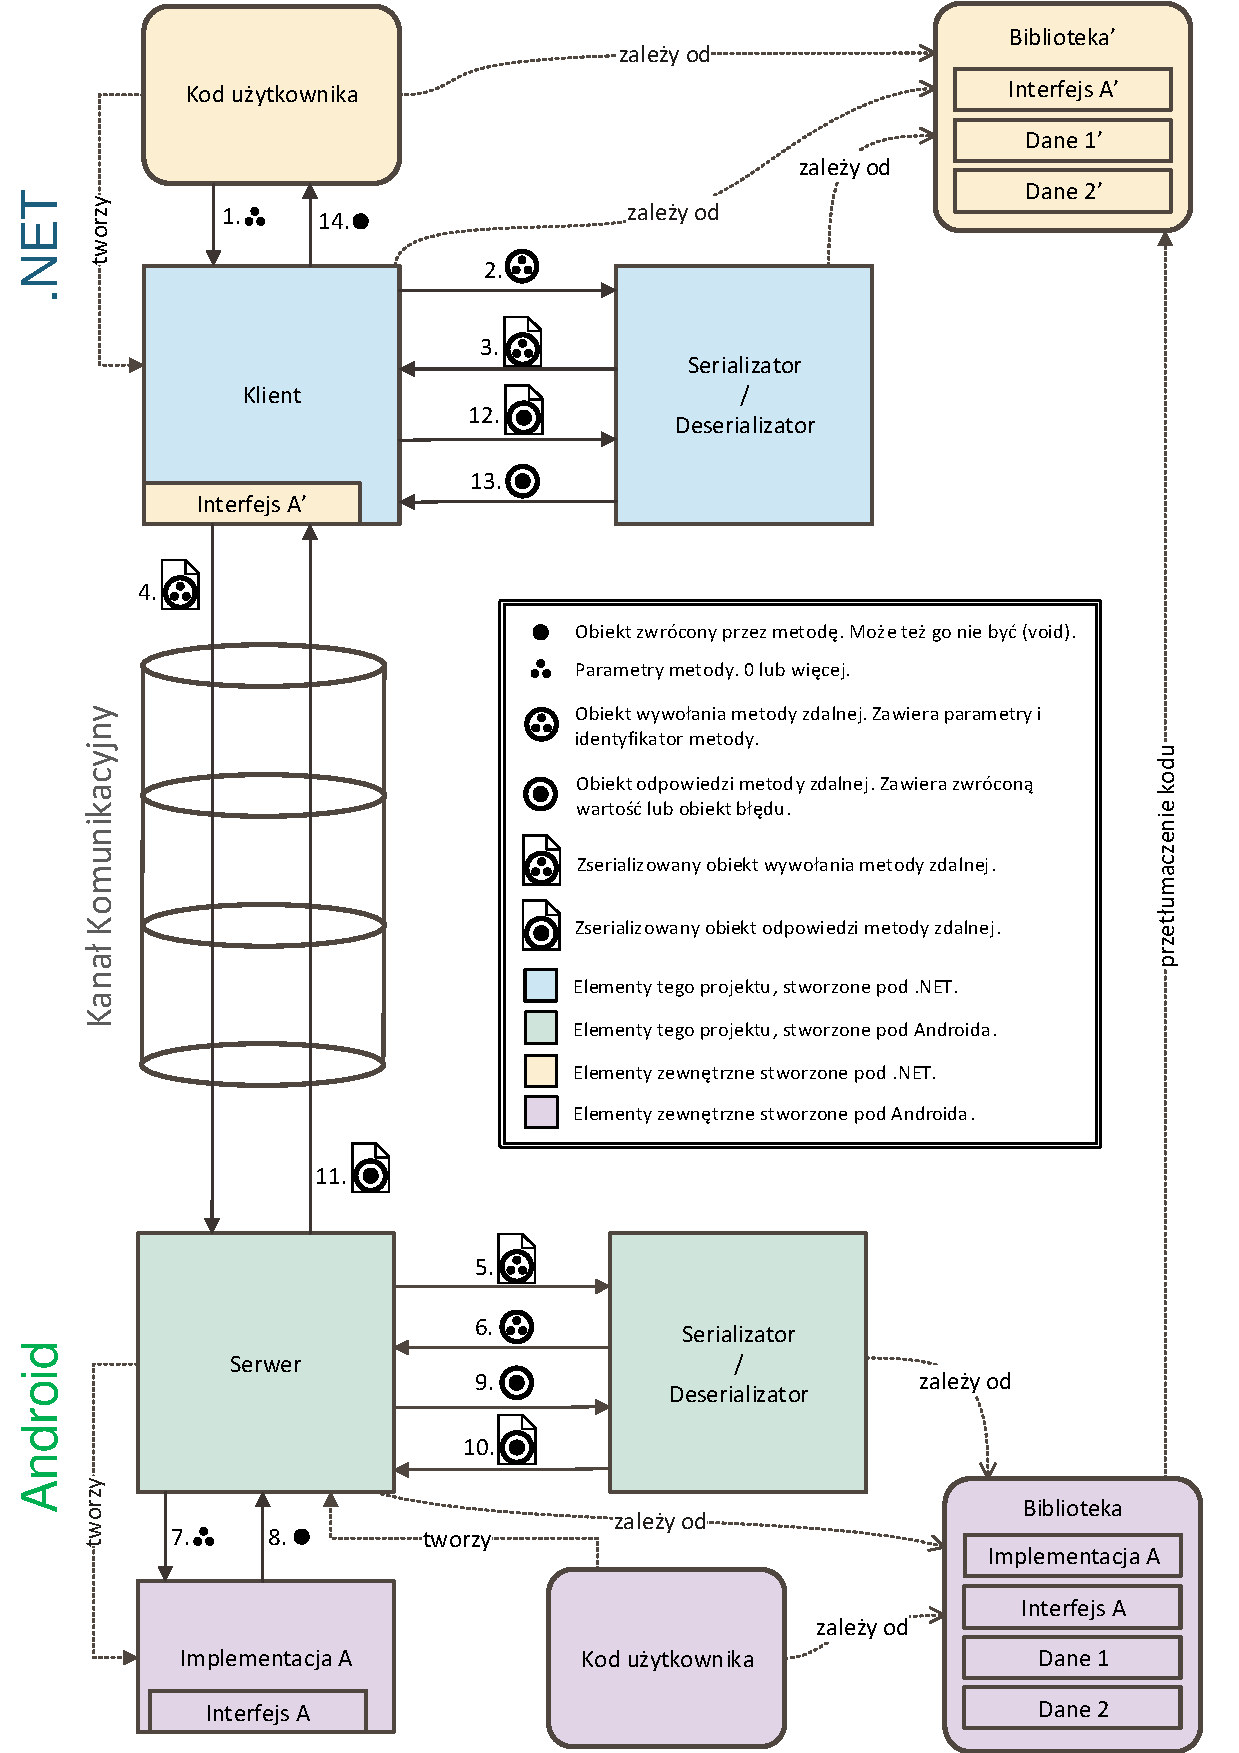
\includegraphics[scale=0.8]{img/schematy/schemat-dzialania-magisterki.pdf}
	\caption{Ogólny schemat projektu.}
	\label{fig:project-overview}
\end{figure}


\subsubsection{Reprezentacja zawartości informacyjnej}
Nie można właściwie mówić o~zawartości informacyjnej systemu, ponieważ takiej nie będzie.
Przez mój system dane będą jedynie przepływać.


\subsubsection{Opis interfejsów systemowych}
\begin{itemize}
	\item Jako, że to, co tworzę będzie kolekcją bibliotek Javy i~C\# będą one mogły być ładowane, a~ich klasy wykorzystywane przez zewnętrzne aplikacje.
	\item Niezależne narzędzie do generacji kodu będzie opatrzone w~interfejs linii poleceń.
\end{itemize}


\subsection{Wymagania funkcjonalne(TODO)}
%opis tekstowy
%ograniczenia
%wymagania wydajnościowe
%zastrzeżenia projektowe
%diagramy pomocnicze

\subsubsection{Serializacja danych z zachowaniem informacji o typach}
Dane serializowane po obu stronach barykady muszą (kiedy to potrzebne do odczytania, a więc jeśli nie wynika jasno z konktekstu) zawierać informacje umożliwiające deserializację odpowiednich typów.
Deserializacja powinna być komplementarna i z tych zapisów odtwarzać obiekty o odpowiednich typach i z poprawnymi danymi.
Jest to warunkiem dla polimorficznych metod.

\subsubsection{Serwowanie polimorficznych metod zdalnych}
To na Androidzie.

Kod wystawiający metody zdalne musi móc wystawić obiekt nieznanej mu, nieoznaczonej jakoś specjalnie klasy jako serwis (robi to przy pomocy refleksji i jakiegoś ogólnego zestawu zasad). Musi być do tego podany jakiś interfejs.

Wystawianie metod rzez jakiś strumień komunikacyjny, np. socket.


Zdalne metody oraz ich argumenty muszą być polimorficzne.
Czy zdalne metody moga byc przeładowywane?
Sprowadza sie do zachowania informacji o typach
w serializowanych danych. Sprawdzane przez serializacje
i deserializacje jednego obiektu (TestDataB widocznego
jako TestDataA) a nastepnie sprawdzenie,
czy jest taki sam.

\subsubsection{Konsumowanie polimorficznych metod zdalnych}
Klien musi być tworzone dynamicznie do jakiejś arbitralnej zdalnej klasy na określonym strumieniu danych. Czyli musi dynamicznie być tworzony obiekt zgodny z jakimś interfejsem. Odpalanie na nim metod powoduje wywołanie metod zdalnych.

\subsubsection{Komunikacja z systemem Android}
Faktycznie chodzi o możliwość wołania metod z API Androida i wysyłanie Intentów, które są takimi wiadomościami.

\subsubsection{Tłumaczenie kodu}
Zrealizowane jako niezależne narzędzie.
Tłumaczenie kodu zmniejszyłoby nakład pracy programisty, który bez tego musiałby sam stworzyć odpowiadające klasy danych w obu językach.

Klasy ze standardowych bibliotek, które nie znajdują odpowiednika nie muszą być tłumaczone.

Jeśli w danej klasie są inne klasy z zewnętrznej biblioteki, to trzeba też przetłumaczyć te. Trzeba dostarczyć kod wszystkich.
Jeśli jedno ogniwo jest nieprzetłumaczalne to można pominąć pole z ostrzeżeniem.

% WYMAGANIA POMIJANE:
% reliable sessions (w sumie też by mi się przydał jakiś mechanizm, który umożliwi komunikację w niestabilnym środowisku Internetu)
% \url{http://blogs.msdn.com/b/shycohen/archive/2006/02/20/535717.aspx} \\


\subsection{Wymagania niefunkcjonalne(TODO)}
O ile techniczne raczej olewam (odnieść się, do działu. Po prostu ma działać.
Ale zależy mi na satysfakcji użytkownika (programisty) i~na prostym użytkowaniu mojego projektu.

minimalizacja nakładu pracy -- np. minimalizacja kodu

To powiedziawszy, tu są pozostające wymagania:

\subsubsection{Wydajność serwera}
Ponieważ chodzi tylko o sprawdzenie założeń nie musi być duża. Wystarczy wsparcie kilku, powiedzmy 5 klientów na raz.

\subsubsection{Klient w .NET pod Windows}
Metody zdalne z Androida mają być konsumowane przez program działający na platformie .NET pod systemem Windows.

\subsubsection{Rozszerzalność bez ingerencji w oryginalny kod}
Można dodawać klasy dziedziczące po obu stronach nie zmieniając kodu metody, przez które przechodzą funkcjonalność metod.
Czy mozna do serwera i klienta dodac moduł, np.
z nowymi klasami danych dziedziczacymi istniejace
i uzywac ich ze starymi metodami?

\subsubsection{Minimalizacja nakładu pracy programisty}
Kompilacja i używanie biblioteki powinno być proste i~intuicyjne.



\section{Prototypy (TODO)}
Muszę naprawdę wiedzieć czego potrzbuje, w końca praca jest podróżą w nieznane. Zanim zacznę robić schematy jak wszystko ma działać i wyglądać muszę naprawdę wiedzieć, co jest potrzebne.

O, Xtreme Programming! Tu są SPikei -- coś czego mi potrzeba, bo nie jestem pewny jak coś zrobić. Mam dużo opcji, najsensowniej będzie sprawdzić parę rzeczy, żeby coś wybrać.

z racji tego, że projekt jednoosobowy i to ja jestem produkt ownerem i każdym, to nie będzie jako takich releasów i planowani iteracji. iteracje tez bez sensu, bo mam po prostu dostarczyć cały produkt. Chociaz moge sobie tym ustalic priorytety

Create spike solutions to figure out answers to tough technical or design problems. A spike solution is a very simple program to explore potential solutions. Build the spike to only addresses the problem under examination and ignore all other concerns. Most spikes are not good enough to keep, so expect to throw it away. The goal is reducing the risk of a technical problem or increase the reliability of a user story's estimate.

Diagram Spike'a objaśnić w moim zastosowaniu (\url{http://www.extremeprogramming.org/rules/spike.html})
Co to SPIKE? Spike w~Extreme Programming, bodajże, ma za zadanie właśnie sprawdzić czy coś się da zrobić oraz jakie elementy będzie musiało zawierać rozwiązanie.
Spike nie musi być gotowym, działającym w pełni produktem. Ale pokazuje, czy sama zasada działania jest słuszna.


Dobrze, żeby prototypy zawierały te wszystkie elementy, ale chociaż je mockowały.

Tylko sprawdzając coś w~ten sposób mogę się przekonać, jaka droga jest dobra. Można myśleć, że przecież z~opisów bibliotek i~technologii można wywnioskować, do czego się nadają, ale w~praktyce tak nie jest. Jak się pisze konkretne rozwiązanie to czasem się okazuje, że akurat to nie działa.


Może kilka spikeów na kilka kawałków rozwiązania?

Założenia każdego prototypu (Spike'a) krótko na początku scharakteryzuję.

Jak oprę się o~Json-Rpc to będę miał system identyfikacji obiektów i~errory gratis.

\subsection{Prototyp: wspólny format informacji o typach}
Zarówno część na Androidzie jak i~.NET musi tak samo oznaczać typy obiektów w~zserializowanych obiektach.
Jest to podstawa do uzyskania polimorficznych zdalnych metod.
Chcę to zrobić przez dobranie serializatorów po obu stronach i~odpowiednią ich konfigurację. Ewentualnie będę ingerował w~ich kod.

Myślę o~Jackson po stronie Androida i~DataContractJsonSerializer lub JSON.NET po stronie .NET\@.

\subsubsection{Wyniki}
I~co, ma to sens? Udało się?


\subsection{Prototyp: polimorficzne metody zdalne}
Zakładam, że prototyp ze wspólnym formatem danych się udał.
W~tym momencie trzeba ustawić zgodne polimorficzne serializatory zarówno dla klienta jak i~serwera i~wywołać jakąś z~metod, którymi testowałem polimorfizm w~rozdziale~\ref{similar-technologies}.

Myślę o~jsonrpc4j (jeśli Jackson w~pierwszym prototypie się spisał) Androida i JSON-RPC.NET po stronie .NET\@.

\subsubsection{Wyniki}
I~co, ma to sens? Udało się?



\section{Dookreślenie rozwiązania}
\subsection{Wybrana ścieżka (prototyp)}
Który SPIKE (a~ztem którą ścieżkę) wybieram do dalszego rozwinięcia?
Dlaczego?

\subsection{Licencja}
Trzeba decydować o tym szybko (link dlaczego?).

Wybrałem MIT license (sam przeczytałem licencje, a porównanie tutaj http://choosealicense.com/licenses/). Jest przeciwnikiem skomplikowanych przepisów, na które Apache (główny konkurent) zakrawa, a na patentach mi nie zależy (wątpię, żebym jakieś tu miał, poza tym w UE nie można patentować kodu, chyba). MIT jest proste, zapewnia wzmiankowanie mojego nazwiska i umożliwia używanie mojego kodu także w komercyjnych rozwiązaniach.

Używa jej Ruby On Rails i pare innych dużych, znanych projektów.

\subsection{Repozytorium}
Musiałem to wybrać przed rozpoczęciem pisania tej pracy, bo chciałem ją tam przechowywać (backup). Sposób przechowywania źródeł to też ważna rzecz (link).

Nawet w przypadku samego dokumenty pomaga mi śledzić zmiany i rozwój oraz zapewnia kopię zapasową (a więc bezpieczeństwo).

Założyłem repozytorium na GitHubie, którego znam. Jest popularny i wygodny w użyciu. Kod ma być publiczny, więc nie mam problemu. 




\subsection{Przypadki użycia}
Jakie są? Do czego można użyć tego systemu? Jak to jest z tym dynamicznym tworzeniem web serviceów z hierarchii klas?



\subsection{Struktura projektu}
Diagramy warstwowe, komponentowe, klas.

Napisać, co jest potrzebne dla remotingu: jakaś tożsamość, adres obiektu, oznaczenia metod, argumentów. Ogólnie to jest dość proste. (jak w~JSON-RPC, tylko z polimorficznymi typami)

%Budowa powinna pozwolić na łatwe podłączenie warstwy bezpieczeństwa (bezpiecznego kanału)
%
%Call:
%- id obiektu (0 dla tworzenia nowego, wtedy argumentem jest tym)
%- id metody
%- parametry
%
%Response:
%- czy sie udalo
%- obiekt zwrotny, opis błędu przy wywołaniu zdalnej metody lub stacktrace z exceptiona, który wystąpił w metodzie
%
%Id metody:
%składa się z nazwy i aliasów jej parametrów.
%
%Alias:
%typy prymitywne - int, string, itp.
%datacontract - sraka:\#ptaka.daka
%lista - List
%tablica - [int, [[int, [sraka:\#ptaka.daka, itp.
%
%Tłumaczenie aliasów:
%C\# tłumaczy klasy na aliasy, jak przetłumaczy dla jednej metody to dodaje to do słownika, żeby potem robić to od razu.
%Java tłumaczy aliasy na nazwy klas (potem loaderem). Wiąże w słowniku id metody z obiektem metody. Może być metoda przyjmująca jakiś konkretny List, np. ArrayList, ale nie może mieć overloada przyjmującego inny List.
%Kiedy czyścić te słowniki?
%
%Loader:
%Loaduje aliasy DataContractów, klasy javowe, klasy serwisów(?). Czyta sobie jary, szuka adnotacji
%
%Typy danych i serwisy w javie są oznaczone namespaceami, odpowiadających im rzeczy z C\# (DataContracty i interfejsy)
%
%Oddzielić abstrakcje od sposobu transportu. Wyróżnic transport streamowany (serializator dostaje strumień i na niego wali output, możemy tłumaczyć i wysyłać na raz) i nie (trzeba stworzyć całą wiadomość, wtedy wysłać).
%
%Zrobić timeouty na łączenie do serwisu i na operacje. Poczytać więcej o TCP, zobaczyć, czy dobrze można nim sprawdzać, czy trzeba używać PINGa.
%
%Serializujemy wszystkie publiczne pola/ propertiesy albo metody z get / set (to w Javie). Używać jakiś dostępnych już atrybutów do ręcznej konfiguracji wyboru serializowanych elementów.

\subsection{Schemat działania projektu}
Schematy działania, to z liniami życia, diagramami aktywności itp.

\subsection{Plan testów}
Jakie testy akceptacyjne? Jak sprawdzę (lub sprawdziłem), że działa? Na jakiej konfiguracji sprzętowej będę musiał to robić?

Tworzenie grafu w~typów w~xmlu? Są obiekty, które mogą mieć dzieci (tablice, listy). Próbuję wygenerować C\# dla porównania. Zapisuję grafy, które nie działają (w trakcie automatycznych testów). Zrobić wizualizator grafów.

Będę robił Test Driven Development. Daje zazwyczaj dobre programy i~skutkuje w~końcu szybszym wykonaniem projektu, bo nie ma przerw w~prcy związanych z jakimiś dziwnymi bugami.

Logowanie też trzeba dać.

\section{Implementacja}
Jakieś szczegóły ciekawsze implementacji opisać. Może to powinno zastąpić czwarty rozdział?

%Dobrze korzystać z~istniejących standardów. Wprowadzenie nowego standardu nie jest dobrą rzeczą, chyba, że ma się ogromną rzeszę zwolenników lub naprawdę poważne przesłanki (powody). Kto wie, może takie mam. Ale na ogół lepiej kombinować istniejące rozwiązania tak, żeby zewnętrzne komponenty miały szansę na współpracę z nimi.
%
%Pomysły do SPIKEów będę wybierał na bazie doświadczenia (i~przesłanek opisanych poniżej w~\ref{approach-selection}).
%Będę starał się wykorzystać jakieś badane wcześniej technologie. Bo lepiej używać gotowych, dojrzałych komponentów tam, gdzie można. Po co wymyślać koło od nowa?
%Spike'i będę tworzył w~kolejności od tego, który według mnie ma największe prawdopodobieństwo na bycie prototypem ostatecznego rozwiązania.
%Może się nawet udać za pierwszym razem, ale na wszelki wypadek powinienem zrobić kilka. Bo a~nóż się okaże, że mój drugi albo trzeci wybór będzie się zachowywał lepiej.
%
%\subsection{Selekcja podejść}
%\label{approach-selection}
%Jakie podejścia, techniki odrzucam, na jakich się skupię, dlaczego?
%
%\subsubsection{Dlaczego nie chcę pisać serializacji}
%To dużo roboty i~zostało zrobione wiele razy. Jak już to bym wziął istniejący projekt, zrobił fork i~dodał wpisywanie i~odczytywanie informacji o~typach. Może nawet potem bym swoje zmiany dodał do oryginalnego projektu?
%
%\subsubsection{Dlaczego nie Schemy i referencje we wiadomościach}
%Chyba nie zależy mi na referencjach, jak linki do schem w SOAPie. System ma być prosty, wiadomości spójne i pełne. Odniesienia powodują dużo skomplikowanie, które jest zbędne - całe dane powinny być zawarte w wiadomości. A no i ja się nie bawię w schemy, nie przesyłam opisu danych (te są w klientcie i serwerze), przesyłam tylko surowe dane.
%
%\subsubsection{Dlaczego nie REST}
%Nie zależy mi konkretnie na łączności przez internet, a~to jest podstawowym założeniem RESTa.
%Chcę wspierać wiele warst transportowych, nie tylko HTTP. Poza tym parsowanie adresów jest bardziej problematyczne niż proste pobieranie nazw metod.
%
%Będę robił raczej RPC z~JSONem, nie będę udawał RESTa.
%WADL nie jest w~ogólności zbyt potrzebny, bo REST może bez niego żyć.
%
%\subsubsection{Dlaczego nie SOAP}
%Nie uważam, że skomplikowanie SOAPa jest odpowiednie do RPC\@. Wystarczy zobaczyć, jak ciężko jest skomunikowac sie z serwisem w WCF przy pomocy kSOAP - ktos wlozyl w to duzo roboty, a i tak w minimalnie bardziej zaawansowanych (tablice?) przypadkach ciezko sprawic, zeby dzialalo. Tylko duze implementacje na duze platformy daja rade.
%
%W generację WSDLa nie chcę się babrać - skomplikowane.
%
%Namespace'y są ważną rzeczą w SOAPie. Ja twierdzę, że nie są potrzebne w tak rozbudowanej formie. Może być jedno standardowe nazewnictwo z kropkami. Zakładam taki jakby jeden globalny namespace na oba runtime'y (klient i serwer). Fakt, że nawet jedna strona może mieć kilka przestrzeni nazw (parę class loaderów albo assembly cache'y) ale nie chcę tego robić z uwagi n utrudnienia w integracji (tu można napisać jakby to mogło wyglądać, ale nie trzeba, mogę po prostu to olać).

%\section{Inne SPIKE'i}
%
%\textbf{Serializacja JSONa (raczej samej serializacji nie chcę robić):}
%Przejrzeć specyfikację, zobaczyć, z czym musieli sobie poradzić i wyczaić jak to wszystko mozna odwzorować w JSONie. Obczaić, jak sobie DataContractSerializer (też DataContractJsonSerializer) radzą.
%
%\textbf{portowanie rozwiązań w C na Androida?}
%Axis w~ C? Może częściowe używanie go spod javy. W sumie można sportować też jakieś inne rzeczy. Np.\ pythonowe web service'y (pyro, twisted). Może podpięcie pod gSOAP? Jakieś tłumaczenie JibXem sportowanych rzeczy?
%
%Sprawdzić Python Remote Objects (Pyro) na pythonie 2, 3 (też na warstwie skryptowej Androida). Porównać z Twistedem, napisać o próbach portowania wymaganych bibliotek w C na Androida. \url{http://pythonhosted.org/Pyro4/intro.html#performance}
%
%sl4a, py4a, kompilacja na ubuntu z użyciem NDK i Cythona
%distutils.core zamienić na setuptools w setup.py
%
%\textbf{Zcentralizowane pseudo web servicy (albo nawet i nie)}
%Też potrzebny serializator / deserializator + bindingi. To był ten pomysł, że to komp pinga serwer (Androida), żeby ten sobie pobrał rozkaz i to Android woła web service na kompie. Trzeba by było używać Ksoap albo innego ścierwa. Zobaczyć, czy to w ogóle miałoby sens. Czy tymi Ksoapami da się coś sensownie zrobić.
%
%\textbf{Własny serwer REST}
%Tu dyskusja o implementacji serwera RESTowego na Androidzie \url{https://groups.google.com/forum/?fromgroups=#!topic/android-developers/vgkXg1P8iBg}